\subsection{نتایج}
\subsubsection{Baremetal}
\smalltitle{Build Schema}
\readevents{results/postgres-baremetal-results/hammerdb-schema-build-bare-metal-5-events.csv}
\readreasonbar{results/postgres-baremetal-results/hammerdb-schema-build-bare-metal-5-shootdowns.csv}
\readstrace{results/postgres-baremetal-results/hammerdb-schema-build-bare-metal-5-syscall-usage.csv}
\smalltitle{کرنل 4}
\readevents{results/postgres-baremetal-results/hammerdb-2-users-bare-metal-4-events.csv}
\readreasonpie{results/postgres-baremetal-results/hammerdb-2-users-bare-metal-4-shootdowns.csv}
\readstrace{results/postgres-baremetal-results/hammerdb-2-users-bare-metal-4-syscall-usage.csv}
\smalltitle{کرنل 5}
\readevents{results/postgres-baremetal-results/hammerdb-2-users-bare-metal-5-events.csv}
\readreasonpie{results/postgres-baremetal-results/hammerdb-2-users-bare-metal-5-shootdowns.csv}
\readstrace{results/postgres-baremetal-results/hammerdb-2-users-bare-metal-5-syscall-usage.csv}
\smalltitle{کرنل 6}
\readevents{results/postgres-baremetal-results/hammerdb-2-users-bare-metal-6-events.csv}
\readreasonbar{results/postgres-baremetal-results/hammerdb-2-users-bare-metal-6-shootdowns.csv}
\readstrace{results/postgres-baremetal-results/hammerdb-2-users-bare-metal-6-syscall-usage.csv}
\subsubsection{VM-1}
\smalltitle{Build Schema}
\readevents{results/postgresql-vm1-results/postgres-schema-build-vm1-5-events.csv}
\readreasonbar{results/postgresql-vm1-results/postgres-schema-build-vm1-5-shootdowns.csv}
\readstrace{results/postgresql-vm1-results/postgres-schema-build-vm1-5-syscall-usage.csv}
\smalltitle{کرنل 4}
\readevents{results/postgresql-vm1-results/postgres-vm1-4-events.csv}
\readreasonbar{results/postgresql-vm1-results/postgres-vm1-4-shootdowns.csv}
\readstrace{results/postgresql-vm1-results/postgres-vm1-4-syscall-usage.csv}
\smalltitle{کرنل 5}
\readevents{results/postgresql-vm1-results/postgres-vm1-5-events.csv}
\readreasonbar{results/postgresql-vm1-results/postgres-vm1-5-shootdowns.csv}
\readstrace{results/postgresql-vm1-results/postgres-vm1-5-syscall-usage.csv}
\smalltitle{کرنل 6}
\readevents{results/postgresql-vm1-results/postgres-vm1-6-events.csv}
\readreasonpie{results/postgresql-vm1-results/postgres-vm1-6-shootdowns.csv}
\readstrace{results/postgresql-vm1-results/postgres-vm1-6-syscall-usage.csv}
\subsubsection{Pages Huge}
\smalltitle{Build Schema}
\readevents{results/postgres-huge2m-results/postgres-huge2m-schema-events.csv}
\readreasonbar{results/postgres-huge2m-results/postgres-huge2m-schema-shootdowns.csv}
\readstrace{results/postgres-huge2m-results/postgres-huge2m-schema-syscall-usage.csv}
\smalltitle{کرنل 4}
\readevents{results/postgres-huge2m-results/postgres-huge2m-4-events.csv}
\readreasonpie{results/postgres-huge2m-results/postgres-huge2m-4-shootdowns.csv}
\readstrace{results/postgres-huge2m-results/postgres-huge2m-4-syscall-usage.csv}
\smalltitle{کرنل 5}
\readevents{results/postgres-huge2m-results/postgres-huge2m-5-events.csv}
\readreasonbar{results/postgres-huge2m-results/postgres-huge2m-5-shootdowns.csv}
\readstrace{results/postgres-huge2m-results/postgres-huge2m-5-syscall-usage.csv}
\smalltitle{کرنل 6}
\readevents{results/postgres-huge2m-results/postgres-huge2m-6-events.csv}
\readreasonbar{results/postgres-huge2m-results/postgres-huge2m-6-shootdowns.csv}
\readstrace{results/postgres-huge2m-results/postgres-huge2m-6-syscall-usage.csv}
\subsection{تحلیل}
در ابتدا از نحوه‌ی کارکرد
\lr{PostgreSQL}
شروع کنیم. در صورتی که به
\lr{syscall}ها
نگاه کنید متوجه می‌شوید که در همه‌ی حالت دو
\lr{syscall}
\link{https://linux.die.net/man/2/pwrite64}{pwrite64} و \link{https://linux.die.net/man/2/sync_file_range}{sync\_file\_range}
بیشترین استفاده را دارند.
\lr{pwrite64} یک \lr{file descriptor}
می‌گیرد و یک بافر را بدون تغییر دادن
\lr{file offset}
در جایی از فایل می‌نویسید. این موضوع عملا ما را از دستور
\link{https://man7.org/linux/man-pages/man2/lseek.2.html}{lseek}
بی‌نیاز می‌کند. همچنین دیگر نیازی به گرفتن
\lr{lock}
برای تغییر
\lr{offset} و سپس نوشتن
نیست.
دلیل این موضوع این است که
\lr{PostgreSQL}
برخلاف چیزی که شاید به نظر برسد از
\lr{page cache}
استفاده می‌کند! این موضوع سرعت خواندن را به شدت زیاد می‌کند ولی یک مشکلی را نیز به وجود می‌آورد.
اگر موقع نوشتن برق قطع شود یا اینکه مشکلی برای هارد به وجود آید
\lr{data loss}
به وجود می‌آید. برای همین
\lr{PostgreSQL}
از تکنیکی استفاده می‌کند که بعد از نوشتن قسمت‌هایی از فایل بلافاصله با
\lr{sync\_file\_range}
آن قسمت را در دیسک نیز می‌نویسد. با این کار هم
\lr{page cache}
را نگه می‌داریم که سرعت خواندن از دیسک بسیار زیاد شود و هم اینکه مشکل
\lr{data loss}
را رفع می‌کنیم چرا که عملا یک
\lr{write through cache}
می‌سازیم. همچنین لازم به ذکر است که برای خواندن نیز از دستور
\link{https://linux.die.net/man/2/pread64}{pread64}
استفاده می‌شود که از لاک کردن بی‌نیاز شویم.

یکی دیگر از نکاتی که باید به آن توجه کنیم استفاده از
\link{https://www.postgresql.org/docs/current/wal-intro.html}{\lr{Write Ahead Logging}}
در
\lr{PostgreSQL}
است. به صورت کلی
\lr{WAL}
قبل از اینکه دیتا را در بلاک‌های مربوط به خود دیتابیس ذخیره کند و یا تغییراتی را در آن
بلاک‌ها بدهد، در یک فایل لاگ تغییراتی که قرار است بدهد را به صورت
\lr{sequentially}
می‌نویسد و در زمان های منظم این تغییرات را اعمال می‌کند. دلیل استفاده از این موضوع دو چیز است.
اول از همه اینکه زمانی که در دیتابیس
\lr{transaction}
می‌زنیم ممکن است که وسط آن منصرف شویم و نیاز به
\lr{rollback}
داشته باشیم. در صورتی که دیتا را در خود دیسک اعمال کنیم،
\lr{rollback}
کرد کار بسار سختی است چرا که هم می‌توان وسط
\lr{rollback}
به اروری بر خورد و هم اینکه باید جایی بالاخره چیز‌هایی که عوض شده است را نگه داشت. اما در صورتی که از
\lr{WAL}
استفاده کنیم، برای
\lr{rollback}
کردن کافی است که لاگ را پاک کنیم! همچنین در صورتی که
\lr{transaction commit}
شود می‌توان در ابتدا تمامی
\lr{pwrite}ها
را انجام داد و سپس با یک دستور
\link{https://man7.org/linux/man-pages/man2/fsync.2.html}{fsync}
محتوای فایل را با دیسک
\lr{sync}
کرد. (دقت کنید که هیچ گاه \lr{fysnc} در \lr{syscall}های زیاد استفاده شده نیامده است ولی در صورتی که فایل 
\lr{csv}
تمام
\lr{syscall}ها
را باز کنید متوجه می‌شوید که چندین بار از
\lr{fysnc}
استفاده شده است.)
همچنین به عنوان یک
\lr{side note}
اگر تست‌های
\lr{schema build}
را نگاه کنید متوجه می‌شوید که در آنجا
\lr{fysnc} و \link{https://linux.die.net/man/2/fdatasync}{fdatasync}
بیشتر استفاده شده است. دلیل این موضوع این است که
\lr{HammerDB}
در تراکنش‌هایی دیتا‌های
\lr{warehouse}
را در دیتابیس می‌نویسد.
یکی دیگر از نکاتی که باید توجه کرد این است که اگر وسط نوشتن برق برود، از آنجا که یک لاگ داریم
می‌توان تمامی کار‌ها را از اول
\lr{replicate}
کرد و با این کار مشکل
\lr{data integrity}
حل می‌شود. همچنین یکی از
\lr{optimize}هایی
که داک
\lr{PostgreSQL}
به آن اشاره می‌کند این است که ممکن است که چندین
\lr{transaction}
را با هم
\lr{fysnc}
کند. با این کار بار دیسک نیز کمتر می‌شود و سرعت برنامه بیشتر می‌شود.

یکی دیگر از نکاتی که از کارکرد
\lr{PostgreSQL}
متوجه شدیم این بود که
\lr{PostgreSQL}
چند ترد مخصوص برای نوشتن دیتا دارد. به عکس
\ref{fig:postgres:results:processes}
توجه کنید. همان طور که می‌بینید دو ترد وجود دارد که یکی
\lr{WAL Writer}
است و دیگری
\lr{Background Writer}.
کار
\lr{WAL Writer}
که مشخص است. فقط نکته‌ای که باید به آن توجه کنید این است که به کمک
\lr{Message Passing}
دیتا بین ترد‌های مختلف جا به جا می‌شود. همچنین این
\lr{Message Passing}
از نوع
\lr{Pipe}
نیست چرا که در
\lr{strace}
ما اثری از
\link{https://man7.org/linux/man-pages/man2/pipe.2.html}{pipe} و \lr{write}
نیست. پس احتمالا این
\lr{message passing}
در سطح
\lr{user space}
انجام می‌شود.
\begin{figure}[H]
    \centering
    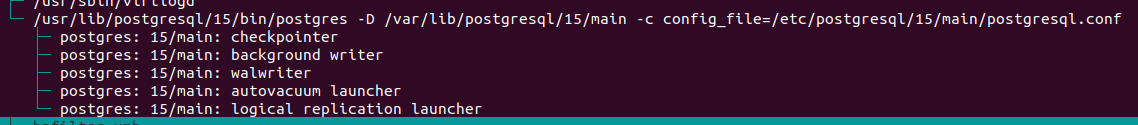
\includegraphics[scale=0.3]{pictures/postgres/results/Processes.png}
    \caption{ترد‌هایی که PostgreSQL ایجاد می‌کند.}
    \label{fig:postgres:results:processes}
\end{figure}
حال به یکی از نکات عجیب برسیم. متوجه می‌شویم که در کرنل نسخه 4 در
\lr{VM} و نه حتی \lr{baremetal}
تعداد
\lr{flush on task switch TLB shootdowns}
به شدت زیاد شده است. این فکت که بر روی
\lr{baremetal}
این اتفاق نیفتاده است مرا به فکر فرو برد که شاید یک
\lr{vulnerability}
در سطح
\lr{CPU}
مثل
\lr{meltdown}
باشد که باعث می‌شود که کل
\lr{TLB flush}
شود. چرا که زمانی که
\lr{meltdown}
پیدا شد برای
\lr{page table isolation}
یا باید کل
\lr{TLB flush}
می‌شد یا اینکه از
\link{https://en.wikipedia.org/wiki/Translation_lookaside_buffer\#PCID}{PCID}
برنامه‌ها در
\lr{TLB}
استفاده می‌کردیم. برای همین موضوع از دستور
\codeword{lscpu}
در ماشین مجازی و محیط
\lr{baremetal}
استفاده کردم. نتیجه‌ی دستور را در محیط
\lr{baremetal}
در کادر زیر و محیط مجازی در شکل
\ref{fig:postgres:results:lscpu:vm}
آورده‌ام.
\codebox{Vulnerability Itlb multihit:     KVM: Mitigation: Split huge pages\\
Vulnerability L1tf:              Mitigation; PTE Inversion; VMX conditional cache flushes, SMT vulnerable\\
Vulnerability Mds:               Mitigation; Clear CPU buffers; SMT vulnerable\\
Vulnerability Meltdown:          Mitigation; PTI\\
Vulnerability Mmio stale data:   Mitigation; Clear CPU buffers; SMT vulnerable\\
Vulnerability Retbleed:          Mitigation; IBRS\\
Vulnerability Spec store bypass: Mitigation; Speculative Store Bypass disabled via prctl and seccomp\\
Vulnerability Spectre v1:        Mitigation; usercopy/swapgs barriers and \_\_user pointer sanitization\\
Vulnerability Spectre v2:        Mitigation; IBRS, IBPB conditional, STIBP conditional, RSB filling, PBRSB-eIBRS Not affected\\
Vulnerability Srbds:             Mitigation; Microcode\\
Vulnerability Tsx async abort:   Not affected}
\begin{figure}[H]
    \centering
    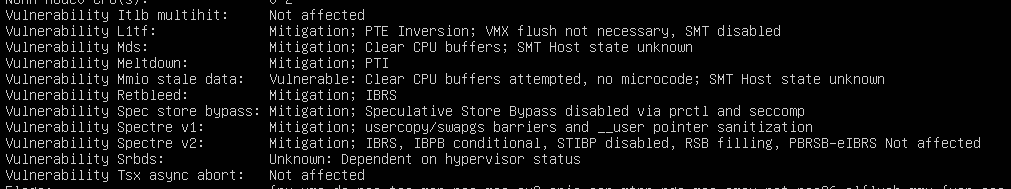
\includegraphics[scale=0.4]{pictures/postgres/results/VM-Vulnerability.png}
    \caption{نتیجه دستور lscpu در VM}
    \label{fig:postgres:results:lscpu:vm}
\end{figure}
در ابتدا به بررسی آسیب پذیری
\lr{Itlb}
پرداخیم. این آسیپ پذیری به نظر می‌آمد که
\lr{VM}ها
را تحت تاثیر قرار دهد و در عین حال مربوط به
\lr{TLB}
است! من با توجه به
\link{https://www.kernel.org/doc/html/next/admin-guide/hw-vuln/multihit.html}{داک}
لینوکس نتیجه گرفتم که احتمالا به خاطر این
\lr{vulnerability}
نیست. دلیل این موضوع یکی این است که این یک مشکل امنیتی است که بر روی
\lr{huge page table}ها
تاثیر می‌گذارد. همچنین
\lr{mitigation}
این موضوع این است که صرفا
\lr{iTLB}
را مجبور می‌کند که از
\lr{page}های
4 کیلوبایتی استفاده کند.
از آنجا که در این تست‌ها
\lr{huge pages}
اصلا روشن نبوده است پس این مشکل امنیتی ما نیست.
اما یک موضوع دیگری اینجا وجود دارد. این مشکل امنیتی نشان می‌دهد که اگر از
\lr{huge pages}
در ماشین مجازی استفاده می‌کردیم احتمالا هیچ بهبودی را نمی‌دیدیم! چرا که در ماشین حقیقی این
\lr{huge pages}ها
به یک
\lr{huge page}
دیگر مپ نمی‌شدند!
کاندید بعدی
\lr{l1tf}
است. این مشکل نیز کاری با
\lr{VMX}
دارد. دوباره در
\link{https://docs.kernel.org/admin-guide/hw-vuln/l1tf.html}{داک}
لینوکس دنبال توضیحات گشتم که این مشکل امنیتی چیست و چه تاثیری می‌گذارد. عبارت
\lr{PTE Inversion}
یک عبارتی بود که به نظر می‌آمد که تاثیراتی را بر روی
\lr{TLB}
بگذارد. ولی با خواندن صفحه‌ی لینک شده به عبارت زیر رسیدیم:
\begin{latin}
\begin{quote}
    The Linux kernel contains a mitigation for this attack vector, PTE inversion, which is permanently enabled and has no performance impact. The kernel ensures that the address bits of PTEs, which are not marked present, never point to cacheable physical memory space.
\end{quote}
\end{latin}
پس عملا این مشکل امنیتی نیز کنار می‌رود و کاری با
\lr{TLB}
ندارد. خود مشکل امنیتی به
\lr{level 1 cache}
کار دارد.

و در آخر می‌رسیم به حمله‌ی
\lr{Meltdown}.
این به صورت خلاصه به کمک سو استفاده از
\lr{speculative execution} و \lr{TLB entries}
می‌تواند که داده‌ای در یک جایی از
\lr{physical memory}
را بخواند. برای رفع این مشکل دو راهکار وجود دارد. یکی اینکه بعد از هر
\lr{context switch} و \lr{userspace} به \lr{kernel space}
رفتن یک
\lr{full TLB flush}
انجام دهیم و دیگری استفاده از
\lr{PCID}
است که
\lr{kernel space} با \lr{user space}
کاملا جدا شود. نکته‌ای که وجود دارد این است که پردازنده‌ی من از
\lr{PCID}
پشتیبانی می‌کند.
\lr{PCID}
از پردازنده‌های نسل چهار به بعد پشتیبانی می‌شود. نه تنها این، بلکه اگر مشکل
\lr{meltdown}
بود چرا در ماشین
\lr{bare metal}
اصلا این اتفاق نیفتاد. اصلا اگر نگاه کنید در کرنل نسخه‌ی 3 در تست
\lr{Sqlite3}
اصلا کلا 9
\lr{TLB shootdown}
داریم! پس قطعا یک مشکلی در
\lr{VM}
بودن وجود دارد که اینقدر
\lr{TLB shootdown}
در حال رخ دادن است. می‌توان سورس کد لینوکس را برای
\lr{source}های \lr{context switch TLB shootdown}
خواند و فهمید که تحت چه شرایطی این اتفاق می‌افتد. اما در حال حاضر نظر ما این است که مشکل امنیتی
وجود دارد که در کرنل 4 درست نشده بود ولی در کرنل‌های بعدی درست شده بود که کرنل 4 مجبور به
\lr{TLB flush}
بود.

یکی دیگر از نکاتی که جا دارد به آن توجه کنیم این است که
\lr{huge pages}
در کرنل نسخه‌ی 6 باعث پایین آمدن فوق العاده زیاد
\lr{TPM}
شد. به همین منظور اجازه دهید که داده‌های
\lr{huge pages}
را تحلیل کنیم. یک چیزی که چشم مرا گرفت ظاهر شدن
\link{https://linux.die.net/man/2/fadvise64}{fadvise64} و \lr{fread64}
در بیشترین
\lr{syscall}هایی
بود که صدا شده بودند. پس من فایل
\lr{strace}
را باز کردم و چک کردم که
\lr{fadvise64}
با چه ارگومان‌هایی در حال صدا زده شدن است. آرگومان آخر که فلگی است که می‌گوید چه کار کند در همه‌ی حالات
\lr{POSIX\_FADV\_WILLNEED}
بود. همچنین حجم
\lr{page}
مورد نیاز همیشه 8 کیلوبایت بود. اما سوالی که وجود دارد این است که چرا اصلا این
\lr{syscall}
اینقدر اسپم شد؟ و همچنین چرا این
\lr{syscall}
در
\lr{VM}ها
نیز زیاد دیده می‌شد ولی در محیط
\lr{bare metal}
دیده نمی‌شد؟ یک چیزی که چشم مرا گرفت این بود که معمولا تعداد
\lr{pread64}
دو برابر تعداد
\lr{fadvise64}
بود. پس احتمالا کل این فرضیه باطل است و صرفا به خاطر
\lr{workload}
این اتفاق افتاده است. اما هنوز معلوم نیست که چرا در کرنل نسخه‌ی 6 این طور سرعت پایین آمده بود.
دو فرضیه وجود دارد. یکی سخت افزار است. اگر می‌شد که بر روی یک سخت فزار دیگر تست کرد خیلی خوب می‌شد.
دیگری مشکل هارد است. ممکن است که هارد من حاوی
\lr{bad sector}
یا مشکلات مشابه بوده باشد. اما این موضوع بعید است چرا که نمودار کاملا
\lr{ramp}
است و به صورت خطی بالا می‌رود. یک فرضیه دیگر است است که کرنل نسخه‌ی 6
(حداقل ورژنی که ما استفاده کردیم)
حاوی باگی است که باعث می‌شود که
\lr{huge pages}ها
بدتر از صفحات عادی عمل کنند. به نظرم این یکی از قسمت‌هایی از آزمایش‌های ما بود که جا دارد که بیشتر
بر روی آن تحقیق کنیم.

در ادامه نیز به برخی اتفاقات
\lr{trivial}
که افتاد می‌پردازیم که بالاخره ذکر کردنشان خالی از لطف نیست. اولین مورد این بود که در کرنل 4 و 5
زمانی که
\lr{huge pages}
را فعال کردیم
\lr{TPM}
ما بهتر شد! این موضوع البته کاملا مورد انتظار بود و همان طور که می‌توانید در جداول مشاهده
کنید تعداد
\lr{dTLB miss}های
ما زمانی که
\lr{huge pages}
را فعال کردیم حدودا نصف شد! چیزی که مرا ناراحت می‌کند این است که این یک
\lr{optimization}
خیلی خوب برای دیتابیس‌ها است ولی در جایی خیلی ندیدم که در مورد این موضوع خیلی حرف زده بشود.
احتمالا دلیل این موضوع این است که این مورد یک
\lr{micro-optimization}
محسوب می‌شود و احتمالا کارای بیشتری مثل عوض کردن
\lr{pool size} و\dots
انجام داد. اما حداقل ما با صرفا فعال کردن
\lr{huge pages}
توانستیم که
\lr{TPM}
خود را تا حدود 25\%
بهتر کنیم. همچنین خیلی تفاوت آنچنانی بین کرنل ورژن 4 و 5 و 6 در محیط
\lr{bare metal}
وجود ندارد و
\lr{TPM}
نسبتا یکسانی به ما می‌دهند.